\section{Task 2 --- Encryption using Different Ciphers and Modes}
%
Firstly, we created a file called {\fontfamily{qcr}\selectfont secret.txt}
containing a secret string ``Hello World!''. Then we created a file
called {\fontfamily{qcr}\selectfont password.txt} containing a password
which is used to derive the actual key for encrypting and
decrypting. In addition, the password stored in {\fontfamily{qcr}\selectfont password.txt}
would be fed into the {\fontfamily{qcr}\selectfont -k flag}, or
{\fontfamily{qcr}\selectfont -kfile flag} if you want only give a filename.
Please note that these two flags are for compatibility with previous versions
of OpenSSL.

In this task, we used Password Key Derivation Function 2 (PBKDF2) with a default number
of iterations for all encrypting/decrypting instances. PBKDF2 is a key
derivation function with variant computational cost,
used to minimize vulnerability to brute-force attacks~\cite{pbkdf2}. PBKDF2 applies
an adittional layer of pseudorandom function, e.g. hash-based message authentication
code, to the given password along with a salt value~\cite{pbkdf2}. By repeating the
process in a number of times to produce a derived key, PBKDF2 makes brute-force attacks
more difficult due to increasing computational work~\cite{pbkdf2}.

In the next subsections, we will discuss how to use OpenSSL to encrypt
and decrypt files with different modes of cipher.

\subsection{AES--256--CBC}
%
\begin{figure}
    \centering
    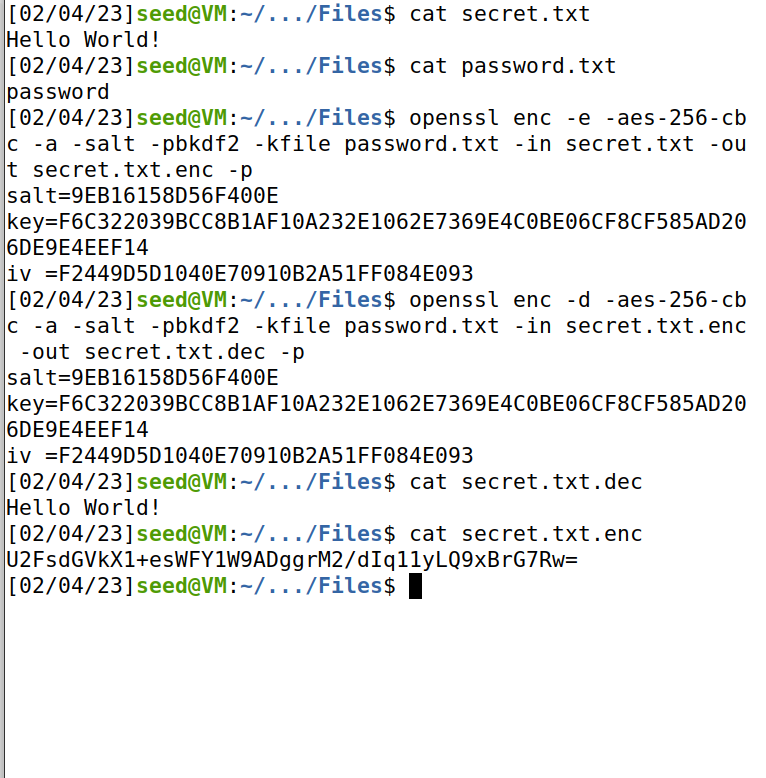
\includegraphics[height=\textheight,width=\textwidth,keepaspectratio]
    {figures/aes-256-enc-dec.png}
    \caption{Encrypting and decrypting a file with OpenSSL AES--256--CBC.}
    \label{fig:openssl_aes_256_cbc}
\end{figure}

Let us explain what was shown in \autoref{fig:openssl_aes_256_cbc}. We executed
the command shown in \autoref{lst:encrypt_openssl} to encrypt a file with
a chosen password which is {\fontfamily{qcr}\selectfont password} in this case.
In that command, we used the following flags and attributes:
\begin{itemize}
    \item {\fontfamily{qcr}\selectfont -e}: encryption mode.
    \item {\fontfamily{qcr}\selectfont -aes-256-cbc}: AES--256--CBC cipher mode.
    \item {\fontfamily{qcr}\selectfont -a}: Base64 process the data.
    \item {\fontfamily{qcr}\selectfont -salt}: Use salt value.
    \item {\fontfamily{qcr}\selectfont -pbkdf2}: Use PBKDF2 algorithm to derive a
    actual key.
    \item {\fontfamily{qcr}\selectfont -kfile file\_name}: Read the password to
    derive the key from the first line of {\fontfamily{qcr}\selectfont file\_name}.
    \item {\fontfamily{qcr}\selectfont -in file\_name}: input file.
    \item {\fontfamily{qcr}\selectfont -out file\_name}: output file.
    \item {\fontfamily{qcr}\selectfont -p}: Display the derived key, salt value, and
    initial vector (IV).
\end{itemize}

At the encryption stage, the {\fontfamily{qcr}\selectfont input file} is a
file containing the secret message, {\fontfamily{qcr}\selectfont secret.txt}.
{\fontfamily{qcr}\selectfont output file} is a file containing the encrypted
message, {\fontfamily{qcr}\selectfont secret.txt.enc}. After running the command
shown in \autoref{lst:encrypt_openssl}, we obtained the following values:

\begin{itemize}
    \item \emph{key = F6C322039BCC8B1AF10A232E1062E7369E4C0BE06CF8CF585AD206DE
    9E4EEF14}
    \item \emph{salt = 9EB16158D56F400E}
    \item \emph{iv = F2449D5D1040E70910B2A51FF084E093}
    \item \emph{Encrypted Message = U2FsdGVkX1+esWFY1W9ADggrM2/dIq11yLQ9xBrG7Rw=}
\end{itemize}

\begin{lstlisting}[language=Bash, caption=Encrypting a file using OpenSSL
    , label={lst:encrypt_openssl}]
$ openssl enc -e -aes-256-cbc -a -salt -pbkdf2 -kfile password.txt \
-in secret.txt -out secret.txt.enc -p
\end{lstlisting}

\begin{lstlisting}[language=Bash, caption=Decrypting a file using OpenSSL
    , label={lst:decrypt_openssl}]
$ openssl enc -d -aes-256-cbc -a -salt -pbkdf2 -kfile password.txt \
-in secret.txt.enc -out secret.txt.dec -p
\end{lstlisting}

In the decryption command shown in \autoref{lst:decrypt_openssl}, a flag
of decryption mode {\fontfamily{qcr}\selectfont -d} was used instead of
{\fontfamily{qcr}\selectfont -e}. As a result, the decrypted text which was
stored in {\fontfamily{qcr}\selectfont secret.txt.dec}, shown in
\autoref{fig:openssl_aes_256_cbc}, was same as the original text ``Hello World!''.

\subsection{DES--CFB}
%
\begin{figure}
    \centering
    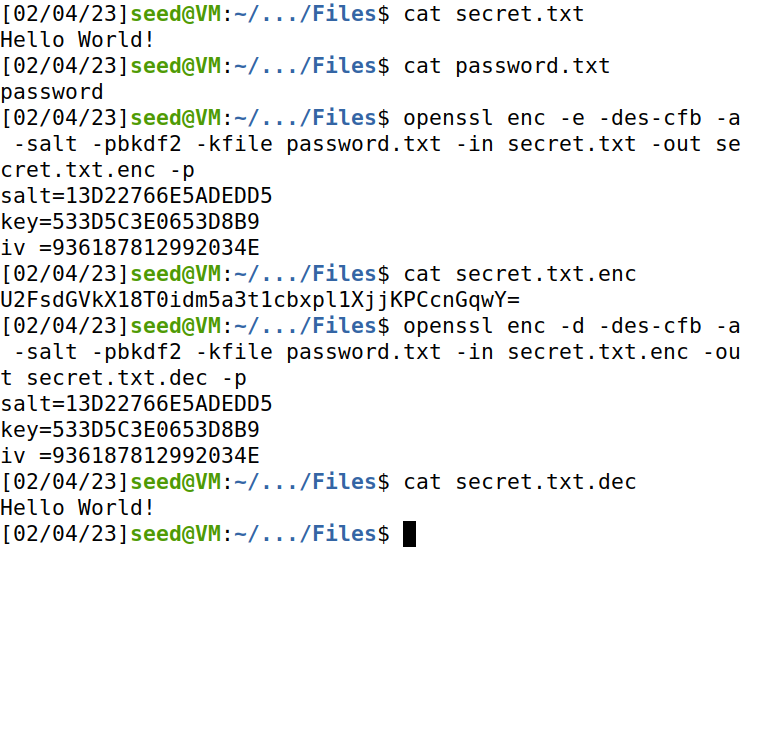
\includegraphics[height=\textheight,width=\textwidth,keepaspectratio]
    {figures/des-cfb-enc-dec.png}
    \caption{Encrypting and decrypting a file using OpenSSL DES--CFB.}
    \label{fig:openssl_des_cfb}
\end{figure}

As shown in \autoref{fig:openssl_des_cfb}, we used the cipher mode
{\fontfamily{qcr}\selectfont -des-cfb}. After running commands shown
in \autoref{fig:openssl_des_cfb}, we obtained the following values:

\begin{itemize}
    \item \emph{key = 3978E9F72DAF7745}
    \item \emph{salt = CFB22A1F393D55AE}
    \item \emph{iv = 49BC3F122B0AD63D}
    \item \emph{Encrypted Message = U2FsdGVkX18T0idm5a3t1cbxpl1XjjKPCcnGqwY=}
\end{itemize}

As a result, the decrypted text was same as the original text ``Hello World!''.

\subsection{BF--ECB}
%
\begin{figure}
    \centering
    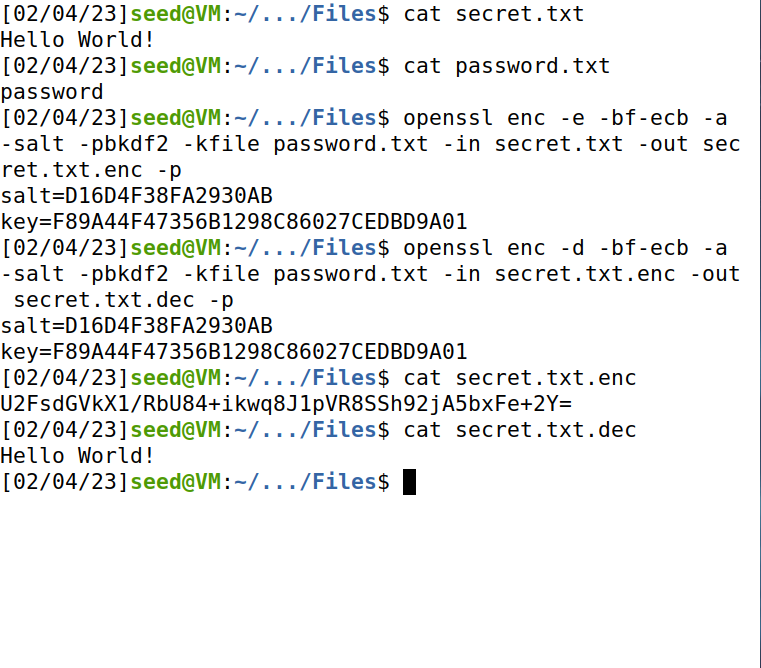
\includegraphics[height=\textheight,width=\textwidth,keepaspectratio]
    {figures/bf-ecb-enc-dec.png}
    \caption{Encrypting and decrypting a file using OpenSSL BF--ECB.}
    \label{fig:openssl_bf_ecb}
\end{figure}

As shown in \autoref{fig:openssl_bf_ecb}, we used the cipher mode
{\fontfamily{qcr}\selectfont -bf-ecb}. After running commands shown
in \autoref{fig:openssl_bf_ecb}, we obtained the following values:

\begin{itemize}
    \item \emph{key = F89A44F47356B1298C86027CEDBD9A01}
    \item \emph{salt = D16D4F38FA2930AB}
    \item \emph{Encrypted Message = U2FsdGVkX1/RbU84+ikwq8J1pVR8SSh92jA5bxFe+2Y=}
\end{itemize}

As a result, the decrypted text was same as the original text ``Hello World!''.